\section{Experiment 3: Adding semantic noise}

% Corresponding Progress Reports
% https://www.notion.so/241025-Matthias-Exploration-of-adversarial-augmentation-199ccb0746f74fd696b8bebe8590fe15
% https://www.notion.so/241101-Matthias-Using-Adversarial-perturbation-to-augment-clip-vision-input-in-Brain-Diffuser-3e8235a27e3c4f4eb67f61a467fd5ada
% https://www.notion.so/241108-Matthias-further-exploration-of-perturbations-196925e9c9b94c04be7a7d1891ce5389?pvs=23
% https://www.notion.so/241114-matthias-Brain-Diffuser-perturbation-big-analysis-13cb45eff9104ae1929522dcf1d39bb9?pvs=23
% https://www.notion.so/250228-Matthias-Filling-the-gaps-5-1a4726ec52d6806e8964f852e5396dc1

% How to execute the whole advpert process?
% 1. Execute multi_process_pert_generation.py (it will generate perturbations for all conditions)
% 2. Execute re_recon_main.py (it will do the reconstructions for all cases -> make sure all data is ready before, baseline needs to be computed beforehand)
% 3. Execute quantitative_eval.py (extracts the quantitative measures from all predicted features/imates)
% 4. Execute create_dfs_advpert.py (creates the dataframes to evaluate the results)
% 5. Execute the analysis_advpert.py (generates the plots)
% 6. For the additional validation plots, execute clip_module_testing.py


\subsection{Background}
Since it was shown in the previous experiment that the CLIP Text features have an influence on the reconstructions only when the mixing in the versatile diffusion process is very high, the next experiment will focus on the influence and possible improvement of the CLIP Vision features. As described above, the number of participants (and the number of images shown to each participant) during the experiment cannot be easily increased, so in this experiment a method will be explored, which modifies the training images in such a way that the diversity of the data can be deliberately influenced without adding new images. Since the measured brain activity was generated in response to the stimuli shown during the experiment, the data enrichment approach chosen for this work should change the images on a visual level as little as possible. The aim of this is that if the enriched images would have been shown in an experiment, it could be assumed that the brain activity recorded for them would be at least very similar to the activity in response to the images that have actually been shown (because a subject would not recognise any difference to the original image). It should therefore be possible to use the already recorded brain activity to train the translator with the enriched images. To effectively alter the results of the trained translator, the embeddings generated by the CLIP Vision encoder from the enriched images (i.e., the translator's training data) must differ from those of the original images, even if the visual appearance remains unchanged. In short, the objective is to modify the CLIP Vision embeddings of input images in a targeted way while preserving their visual similarity to the original. To achieve this, this work will employ adversarial perturbations~\cite{goodfellowExplainingHarnessingAdversarial2014, papernotPracticalBlackBoxAttacks2017, naseerIntriguingPropertiesVision2021}.

Adversarial perturbations are small changes to the input data that are almost invisible to humans, but have a large impact on the internal representation of the input in a machine learning model. For white-box perturbations (such as FGSM~\cite{goodfellowExplainingHarnessingAdversarial2014}), knowledge of the used model, its parameters, gradients and architecture is required. Black box methods do not require any knowledge of the model, so at best they can deceive a wide range of models~\cite{papernotPracticalBlackBoxAttacks2017}. This study uses the CLIP Vision model as the encoder, which is based on a vision transformer architecture~\cite{dosovitskiyImageWorth16x162021}. Although vision transformers have proven to be comparatively robust against adversarial perturbations, they are still susceptible to gradient-based white-box perturbations~\cite{naseerIntriguingPropertiesVision2021}. It can therefore be assumed that, even though the perturbations would not generalise across different models, it's feasible to create perturbations for our purpose, since full knowledge of the model is available. As in the previous experiment of this paper, the multimodality of the CLIP model can be used here to perturb an input image via the CLIP Vision encoder using embeddings created with the CLIP Text encoder. In this way, `semantic noise' can be introduced into the images, which steers the CLIP Vision encodings of the perturbed images in a particular direction guided by the chosen CLIP Text embeddings. The basic procedure of the perturbations is illustrated in Figure~\ref{fig:perturbation_example}: The input image of a dog is easily recognised as such by the CLIP Vision encoder. However, if a gradient-based perturbation containing the semantic information `cat' is applied to the image  (encoded using CLIP Text), the CLIP Vision encoder now has significantly more difficulties identifying the image and might be more likely to see a cat in the image. However, to the human eye the perturbed image look almost identical to the original image.

\begin{figure}[ht]
    \centering
    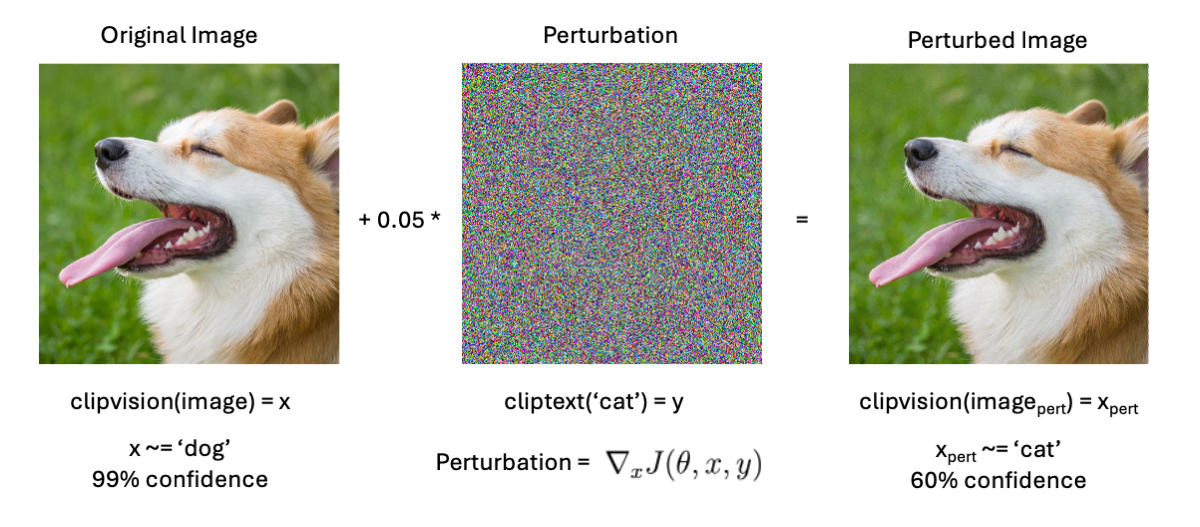
\includegraphics[width=0.8\textwidth]{plots/peturbation_example.png}
    \caption[Example of the perturbation process]{Example of the perturbation process. During the perturbation, the original image is added with slight noise, that the model would identify as a different object. The result is a perturbated image that looks very similar to the original image to the human eye, but the embedding from CLIP vision is altered drastically.}\label{fig:perturbation_example}
\end{figure}

Adversarial perturbations have often been used in the past to enrich training data~\cite{goodfellowExplainingHarnessingAdversarial2014,madryDeepLearningModels2019}. In particular, the goal was to increase robustness against adversarial attacks. Sometimes, this so-called adversarial training degrades the generalisation of the model in the real input space~\cite{kurakinAdversarialMachineLearning2017}. On the other hand, there are results showing that a deliberate enrichment of the training dataset with perturbed data may improve the performance and generalization ability on the test dataset~\cite{xieAdversarialExamplesImprove2020}.  In another study on MRI data of knees, training data was partially augmented with the FGSM algorithm to successfully improve a classification task~\cite{yanEnhancingClassificationPerformance2023}. Overall, there is a mixed picture as to whether adversarial perturbations can be successfully used to enrich training data. However, to the best of our knowledge, there has been no attempt to use targeted white-box perturbation to introduce (or decrease) semantic information into training data to improve the training of ML models such as our Translator module. 

% Durch das Hinzufügen einer weiteren fiktiven Target Domain konnte die Domain Adaptation von generativen Modellen mitunter auch verbessert werden~\cite{volpiAdversarialFeatureAugmentation2018}.

In our experiment, semantic perturbations are created in two different ways: in the first condition, perturbations are used to insert valid semantic information into the original image (e.g.\ a caption describing the bat for an image of a bat); in the second condition, inappropriate semantic information is inserted into the original image (e.g.\ a random caption). The perturbations with valid labels are called `friendly perturbations', the perturbations with invalid labels are called `adversarial perturbations'. Within the perturbation process, the training dataset size can then be increased, by creating multiple perturbed versions of the same input image (using different captions). The  hypothesis is that the friendly perturbations can be used to improve the performance of the \rOne{translator} (and thus the reconstruction) for the natural test images, and the adversarial perturbations can be used to improve the performance of the \rOne{translator} for the artificial shapes. The reason for this is that the friendly perturbations place more emphasis on the semantic meaning in the images and thus the translator learns to recognise these high-level features, which can be helpful with the natural test data that itself contains image with high semantic value. On the other hand, the adversarial perturbations would impair the semantic information, so that the translator would have to use the low-level information that remains in the image, this low-level information should important for the artificial images (as they contain very little semantic information).


\subsection{Methods}

The perturbation procedure is described below. The training images are to be manipulated in such a way that they look almost the same as before while drastically manipulating the semantic information that the CLIP Vision encoder reads from them. Two different algorithms are analysed to generate the perturbations in the images. It is then determined which of the two algorithms is better at achieving the goal of keeping the input image visually as close to the original as possible while at the same time producing different CLIP Vision embeddings. Subsequently, all training data is perturbed using this algorithm and the perturbed versions are used to train the CLIP Vision translator of the Brain-Diffuser algorithm.

\subsubsection{Perturbation process}

% FGSM Algorithm Formula
First, the Fast Gradient Sign Method~\cite{goodfellowExplainingHarnessingAdversarial2014} (FGSM) is used to generate the perturbations. In FGSM, an image is first encoded with a model (here the CLIP Vision encoder) in a forward step, then a loss to a desired output vector the perturbation vector is calculated with respect to the input image, then the sign of the gradient (multiplied by a freely chosen factor $\epsilon$) is subtracted from the input image in a single backpropagation step. This procedure ensures that the CLIP Vision output of the perturbed image is more similar to the perturbation vector. The mathematical description of the algorithm is as follows

\[
x_{pert} \coloneq x + \epsilon \cdot \text{sign}(\nabla_x J(\theta, x, y))
\]

where:
\begin{itemize}
    \item \( x_{pert} \) is the perturbed image,
    \item \( x \) is the original image,
    \item \( y \) is the perturbation vector,
    \item \( \epsilon \) is the perturbation factor,
    \item \( \nabla_x J(\theta, x, y) \) is the gradient of the loss function \( J \) w.r.t.\ \( x \),
    \item \( \text{sign}(\cdot) \) is the element-wise sign function.
    \item \( \theta \) represents the model parameters,
\end{itemize}

In principle, all possible vectors that have the same output format as the CLIP Vision encoder can be used as perturbation vectors. In our case, we take advantage of the multimodality of the CLIP model and can use CLIP Text embeddings as perturbation vectors. In this way, the semantic information from the captions can be partially stored in the images, at best without being highly visible in the images. In our case, two types of captions are inserted into the images via the perturbation: on the one hand, captions are used that represent the valid image in question (friendly perturbations). On the other hand, invalid captions are used, i.e.\ where the caption describes something other than what can be seen in the image (adversarial perturbations). 

% IC Algorithm Formula
In addition to the one-step FGSM algorithm, an iterative perturbation method developed for this work is used. The method will be called Iterative Criterion (IC). Here, too, the input image is systematically adjusted by backpropagation so that the output of the CLIP Vision model of the perturbed input image approach a previously selected perturbation vector. As before, this perturbation vector must be in the same space as in the FGSM algorithm, and again CLIP Text embeddings of friendly and adversarial captions are used. The difference to the FGSM algorithm is that the perturbation is not performed in a single step, but iteratively in several steps until a criterion is reached. The criterion determines how similar (measured by cosine distance) the output of the CLIP Vision embedding of the perturbed image should be to the perturbation vector in comparison to the original image. For example, with a criterion of 50/50, the input image would be perturbed until the CLIP Vision embeddings of the perturbed version have the same cosine distance from the perturbation vector as the original CLIP Vision embeddings (with a criterion of 10/90, until the distance of the perturbed embeddings from the perturbation vector is greater than 11.1\% of the distance of the perturbed embeddings from the original embeddings). In addition, a maximum number of steps is introduced if the algorithm does not reach the target criterion. The formal definition of the algorithm is as follows 

\[
\begin{aligned}
& \textbf{Iteration: For } t = 0 \textbf{ to steps:}\\
& \quad 1.\; y_t = \mathrm{CLIP Vision.encode}(x_t), \\[4pt]
& \quad 2.\; d_{\text{text}} = \cos \bigl(y_t, y_{text} \bigr) \\[4pt]
& \quad 3.\; d_{\text{vision}} = \cos \bigl(y_t, y_{vision} \bigr) \\[4pt]
& \quad 4.\; \textbf{if} \;\frac{d_{\text{text}}}{d_{\text{vision}}} 
\;>\; LC \textbf{ or } t > \text{steps}, \;\textbf{then break}.\\[6pt]
& \quad 5.\; \textbf{else } x_{t+1} 
\;=\; x_t \;-\; \eta \,\nabla_{x_t} (\theta, d_{\text{text}}), \\[4pt]
%
& \textbf{Output: } x_t \quad \text{(perturbed image)}.
\end{aligned}
\]

where:
\begin{itemize}
    \item $\mathbf{x}_0$ is the original input image
    \item $\eta$ is the learning rate
    \item $LC$ is the stop criterion (number between 0 and 1)
    \item $y_t$ is the CLIP Vision encoding of $x_t$
    \item $y_{text}$ is the CLIP Text encoding of the selected caption
    \item $y_{vision}$ is the CLIP Vision encoding of initial input image
    \item cos is the cosine distance
    \item steps is the maximum number of steps to iterate
\end{itemize}

For faster convergence, the learning rate is set to 3 in the first 100 steps, to 1.5 between step 100 and step 300 and then to 1. The maximum number of steps is set to 500.

\subsubsection{Perturbation validation}

In the following, the two perturbation methods will be examined more closely, and it will be determined how well they perform in generating highly modified CLIP Vision embeddings from a largely visually unchanged image. First, however, we will check whether the distinction between friendly and adversarial captions in terms of similarity to the input images works at all. For this purpose, the cosine distance to a friendly and a adversarial caption was measured for all 1200 input images. The results are shown in Figure~\ref{fig:advpert_sanity_check_friendly_vs_adversarial_cap}.

% Image from smith clip_module_testing.py
\begin{figure}[ht]
    \centering
    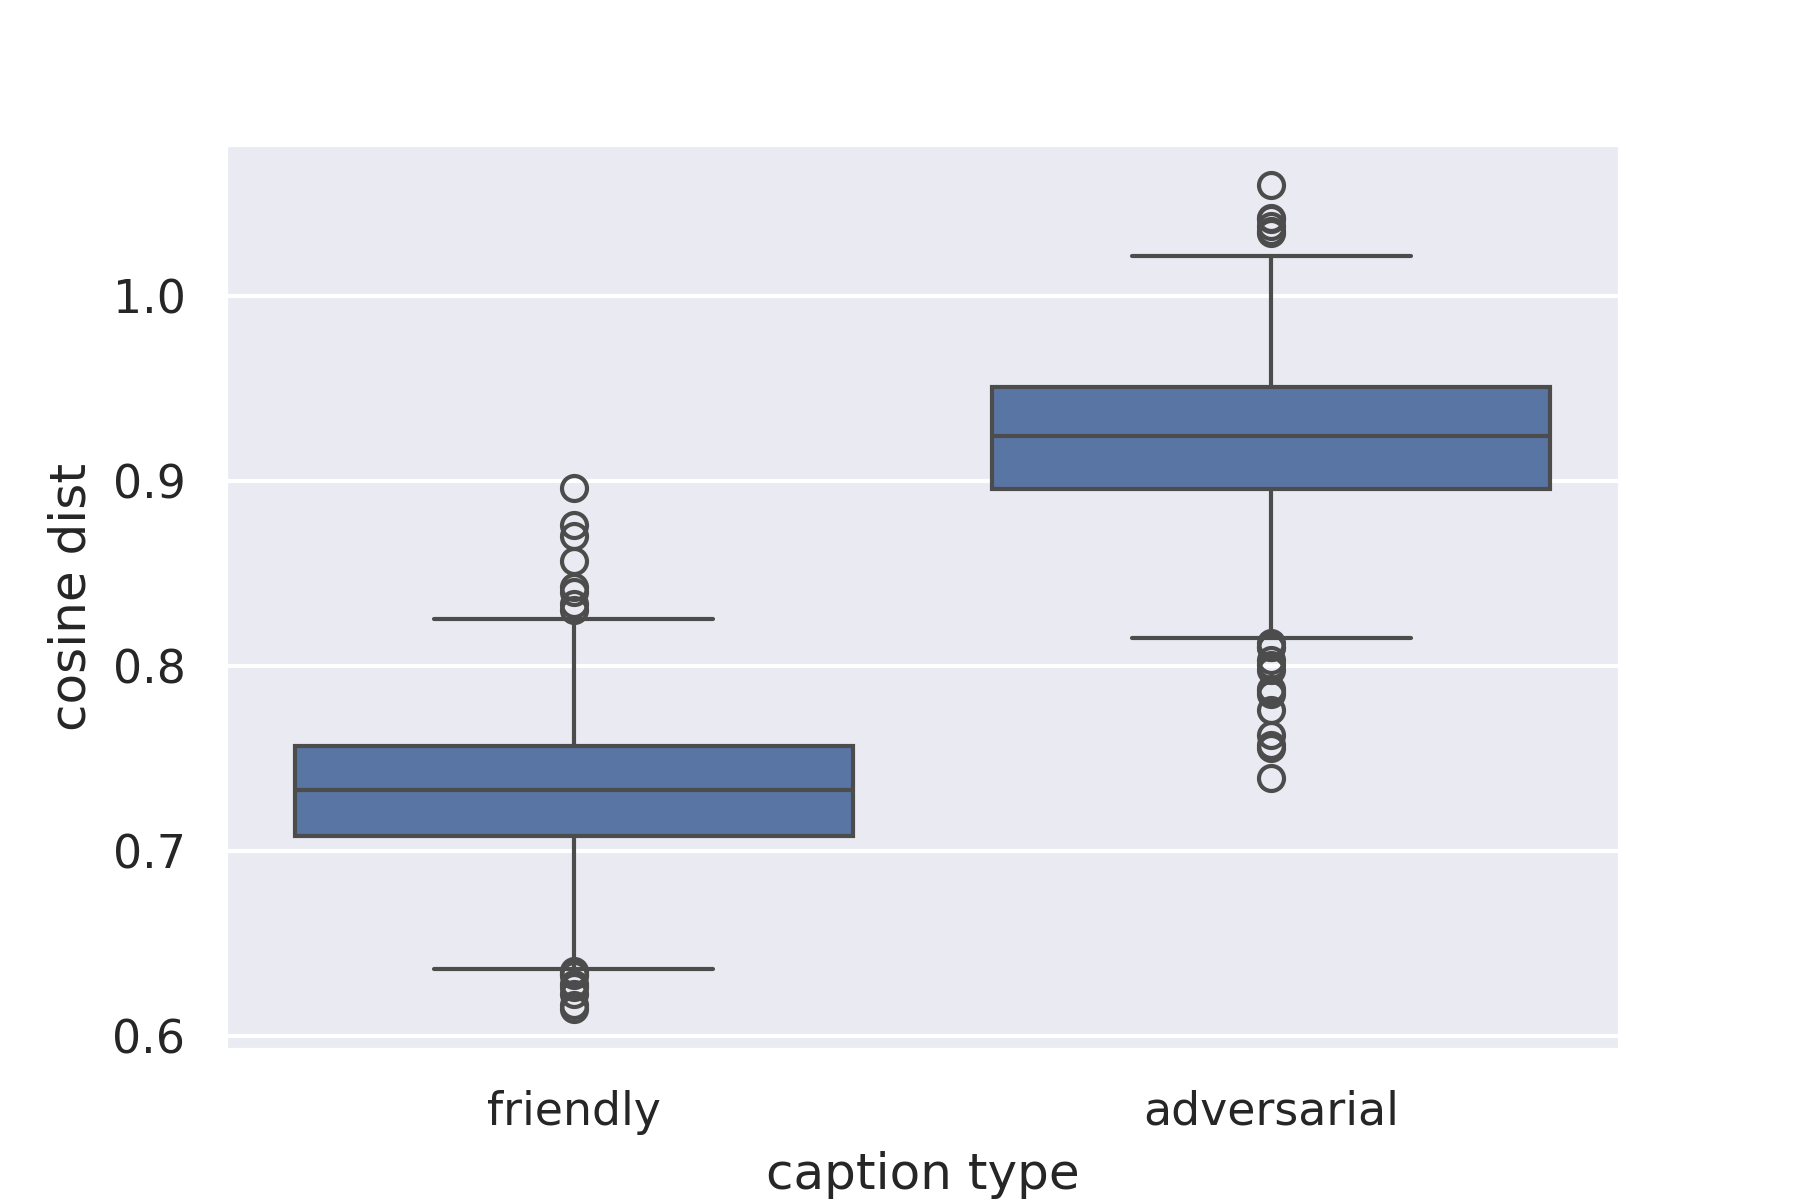
\includegraphics[width=0.6\textwidth]{plots/advpert_sanity_check_friendly_vs_adversarial_cap.png}
    \caption[Similarity of caption embeddings to the respective images]{Distance of friendly and adversarial captions to their respective images. For all training samples, the cosine distance of the CLIP Vision embedding of the image and the CLIP Text embedding of either a friendly (describing the corresponding image) or adversarial caption (describing another image) is computed and displayed in a boxplot.}\label{fig:advpert_sanity_check_friendly_vs_adversarial_cap}
\end{figure}

\noindent{}It is clear that the friendly captions have on average a lower cosine distance to the images (0.74) than the adversarial captions (0.91). It can therefore, as expected, be assumed that friendly captions are more similar to the respective images than adversarial captions. 

In the following, the IC algorithm is examined in detail in a preliminary investigation to determine whether it can achieve the goal of significantly changing the CLIP Vision embeddings while maintaining visually similar images. For this purpose, each of the 1200 input images was perturbed with as many steps until the 50/50 criterion was reached (i.e.\ the cosine distance of the CLIP Vision embeddings to the original image is lower than to the CLIP Text embeddings of the perturbed caption). Additionally, the pixel correlation of the perturbed image to the original image was calculated for each iteration step. The average within a step was calculated for all 1200 input images. The results of this analysis are shown in Figure~\ref{fig:advpert_validation_ic_loss_curves}. 


% Show how the loss is developing for the IC criterion 
% TODO: need an image for that
% Both friendly and adversarial in one image -> To show, that both of them develop similarly
\begin{figure}[ht]
    \centering
    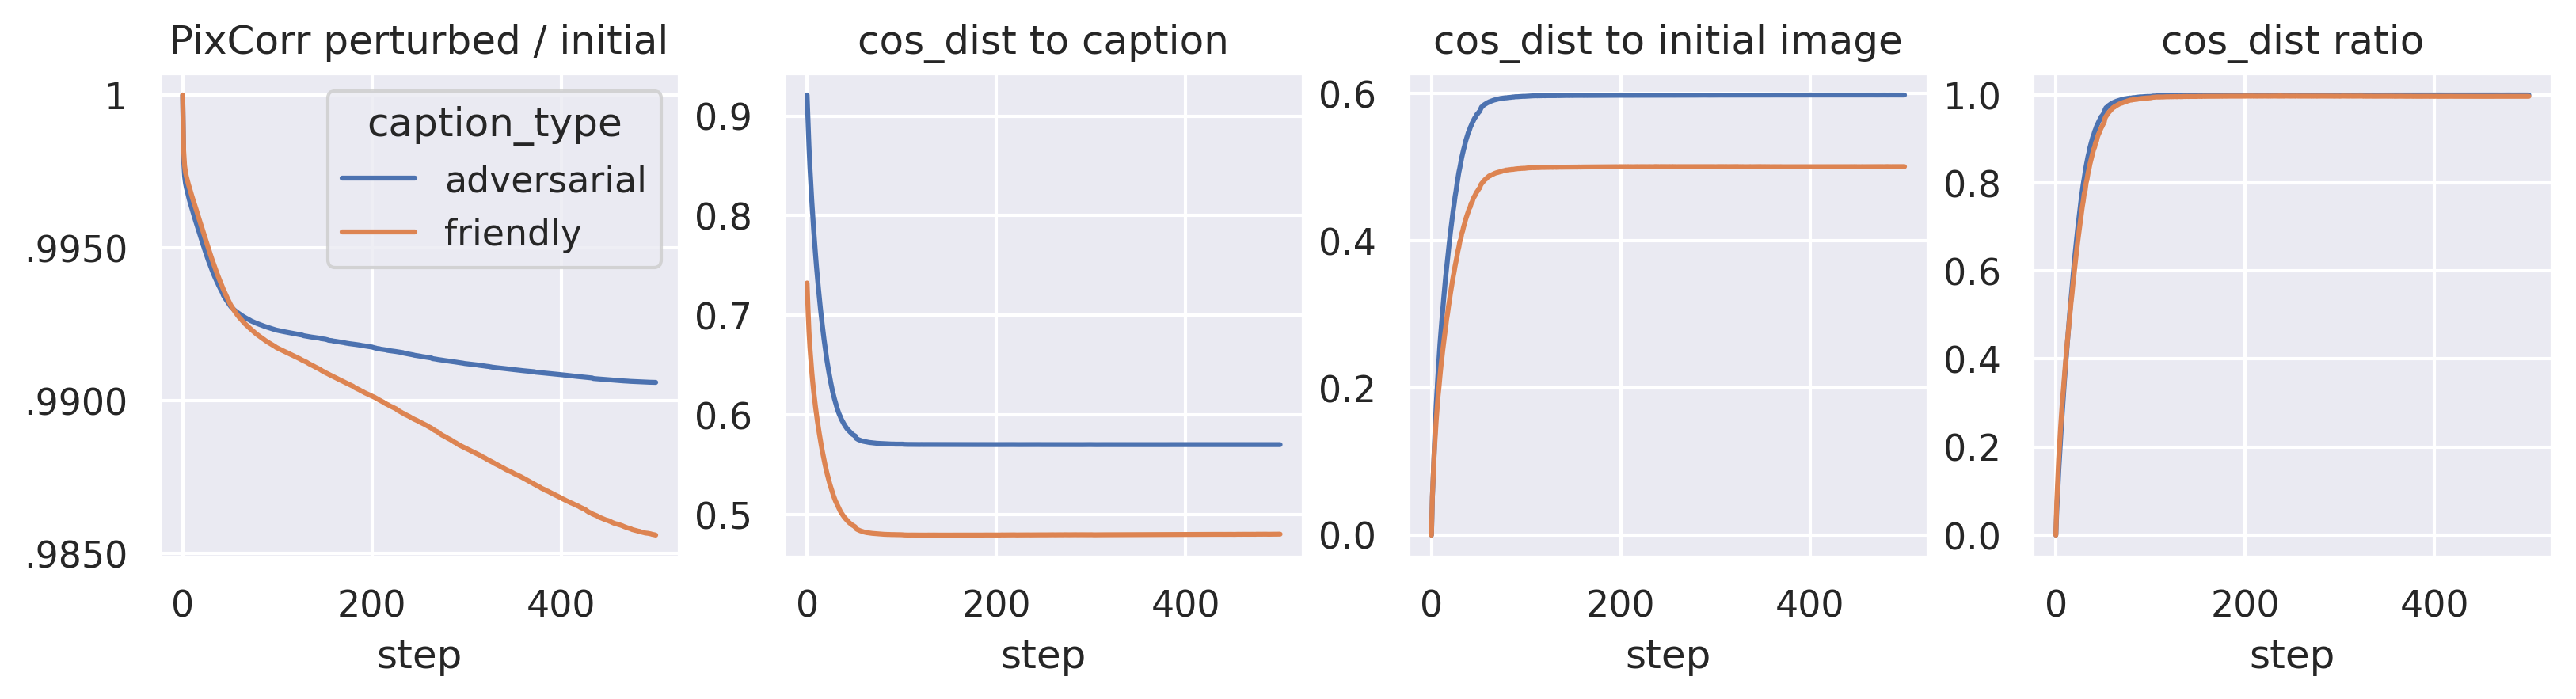
\includegraphics[width=1\textwidth]{plots/advpert_validation_ic_loss_curves.png}
    \caption[Quantitative Evaluation Criteria for the IC Algorithm]{Quantitative Evaluation Criteria for the IC Algorithm. The perturbation using the IC algorithm was performed for all 1200 training samples. Four different criteria are measured at each of the 500 perturbation steps and averaged across all the training samples: The PixelCorrelation of the perturbed and the initial image, the cosine distance of the perturbed image to the caption used for the perturbation process, the cosine distance to the initial image and the ratio of both cosine distances. The perturbation process is stopped, once the ratio reaches 1.0.}\label{fig:advpert_validation_ic_loss_curves}
\end{figure}

The figure shows that the development for adversarial and friendly captions is comparatively similar. The pixel correlation remains very high over time, indicating a relatively small visual deviation from the original image. The cos distance to the perturbation caption decreases continuously with the number of steps, while the cos distance to the original image increases. It can be seen that the cos dist ratio has reached the 50/50 (1) criterion for most images after about 100 steps. As shown before, the initial cos distance of the original images is higher for the adversarial captions than for the friendly captions.

% Show how the results of IC change with more and more epochs (together with the IC loss plot)
    % With images for each epoch

\begin{figure}[ht]
    \centering
    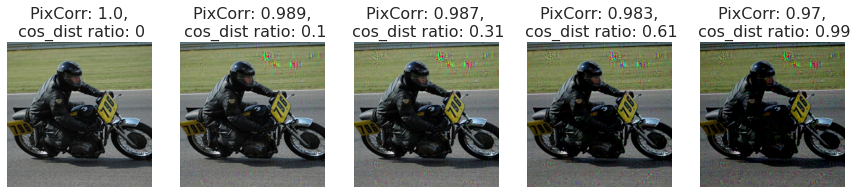
\includegraphics[width=1\textwidth]{plots/advpert_ic_qual_validation_evolution.png}
    \caption[Qualitative Evaluation of Different IC cosine dist ratios]{Qualitative Evaluation of Different IC cosine dist ratios. A snapshot image of the perturbated image is taken for multiple different cosine dist ratios (here loss ratio). The PixelCorrelation and loss ratio are displayed together with the perturbated images at this stage.}\label{fig:advpert_ic_qual_validation_evolution}
\end{figure}

Figure~\ref{fig:advpert_ic_qual_validation_evolution} shows a qualitative representation of how the images change during the perturbation process. It shows the respective pixel correlation to the original image (far left) and the cosine dist ratio explained before. It can be seen that the IC algorithm produces very locally visible perturbations. The majority of the image remains largely untouched, but visual artefacts appear locally. In general, the IC algorithm also seems to have a bias that reduces the brightness of the image if too many perturbation steps are made. Care should therefore be taken in the final experiment not to choose too many perturbation steps in order to maintain the high pixel correlation with the original image. In summary, the IC algorithm is well suited to specifically modify the CLIP Vision embeddings of an image, while the optical alteration, as measured by the pixel correlation, remains comparatively small. In consideration of the analysis of the IC algorithm, the criterion is set to \textbf{80/20} for further experiments. This ensures on the one hand that the perturbation has a noticeable effect on the perturbed images and approaches the CLIP Text embeddings of the selected captions, and on the other hand that the visual perturbation does not become too strong. 


\begin{figure}[ht]
    \centering
    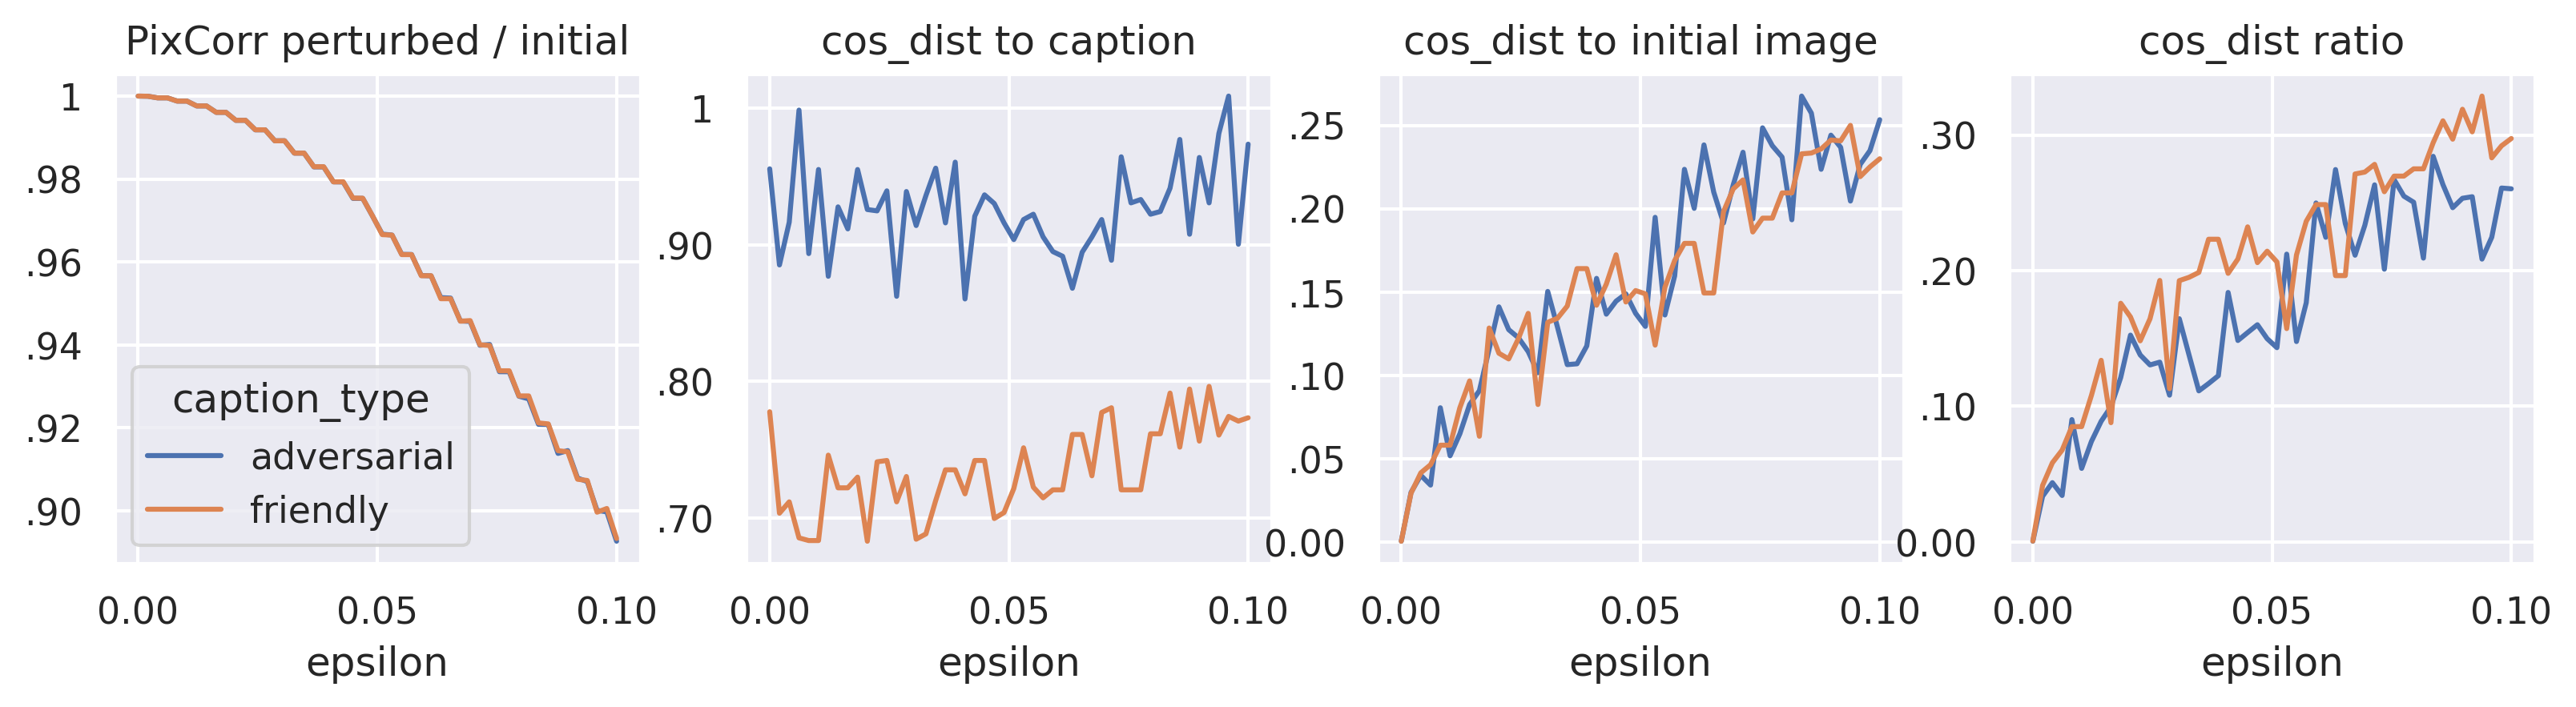
\includegraphics[width=1\textwidth]{plots/advpert_validation_fgsm_loss_curves.png}
    \caption[Quantitative Evaluation Criteria for the FGSM Algorithm]{Quantitative Evaluation Criteria for the FGSM Algorithm. The perturbation using the FGSM algorithm was performed for all 1200 training samples. Four different criteria are measured for multiple epsilons and averaged across all the training samples: The PixelCorrelation of the perturbed and the initial image, the cosine distance of the perturbed image to the caption used for the perturbation process, the cosine distance to the initial image and the ratio of both cosine distances.}\label{fig:advpert_validation_fgsm_loss_curves}
\end{figure}

FGSM is evaluated in the same way as the IC algorithm. Figure~\ref{fig:advpert_validation_fgsm_loss_curves} shows the same metrics as for IC.\@ This time the x-axis shows not the iteration steps but the parameter epsilon, which influences how much the image may be changed in the single perturbation step. Since the FGSM algorithm always changes each pixel by the same value (with a different sign), the pixel change in the image must be exactly the same for the same epsilon (this is indicated by the same pixelCorrelation for both caption types). However, the cosine distance to the perturbation vector (caption) shows that FGSM is not able to approach the desired perturbation vector with increasing epsilon. It can be assumed that the changes here become too large to go in a specific direction in the loss landscape. At least the distance to the original image increases with increasing epsilon, so that the increasing cos dist ratio with increasing epsilon depends mostly on the distance to the original image, but not on the proximity to the desired perturbation vector. 

% Show the influence of friendly vs adversarial perturbation on PixCorr
    % Both for FGSM and for IC
    % -> Not so much changes in the images
    \begin{figure}[ht]
        \centering
        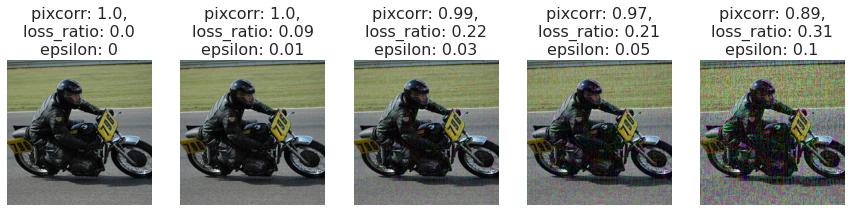
\includegraphics[width=1\textwidth]{plots/advpert_fgsm_qual_validation_evolution.png}
        \caption[Qualitative Evaluation of different FGSM epsilons]{Qualitative Evaluation of different FGSM epsilons. The perturbated image is taken for multiple different epsilons. The PixelCorrelation and loss ratio are displayed together with the perturbated image for each given epsilon.}\label{fig:advpert_fgsm_qual_validation_evolution}
    \end{figure}
    

A qualitative examination of the FGSM results in Figure~\ref{fig:advpert_fgsm_qual_validation_evolution} also shows the difference to the IC algorithm: in contrast to IC, the perturbation is globally visible in the form of noise in the entire image. Local artefacts as in IC are not visible here. In summary, the FGSM algorithm is good at visually changing the image to a predictable extent, but not particularly good at making the perturbation run in a targeted direction. The perturbations here are global and are particularly noticeable as the distance from the original image increases. For further experiments the epsilon is set to \textbf{0.03}. Since a further convergence to the perturbation vectors with an increased epsilon is not to be expected with FGSM, the epsilon is chosen here so that the perturbation has an influence on the image, but does not change the original image too much.

% Define the parameters that will be used in the final test 
    % 80/10 for IC and 0.03 for FGSM

% Show how loss to original CLIPfeatures and caption CLIP features are on average for the chosen perturbations
    % Don't need to show ALL the pictures here I guess? Otherwise I'd have to do the whole perturbation process again
    % oh boy. Oh you poor little boy...
\begin{figure}[ht]
    \centering
    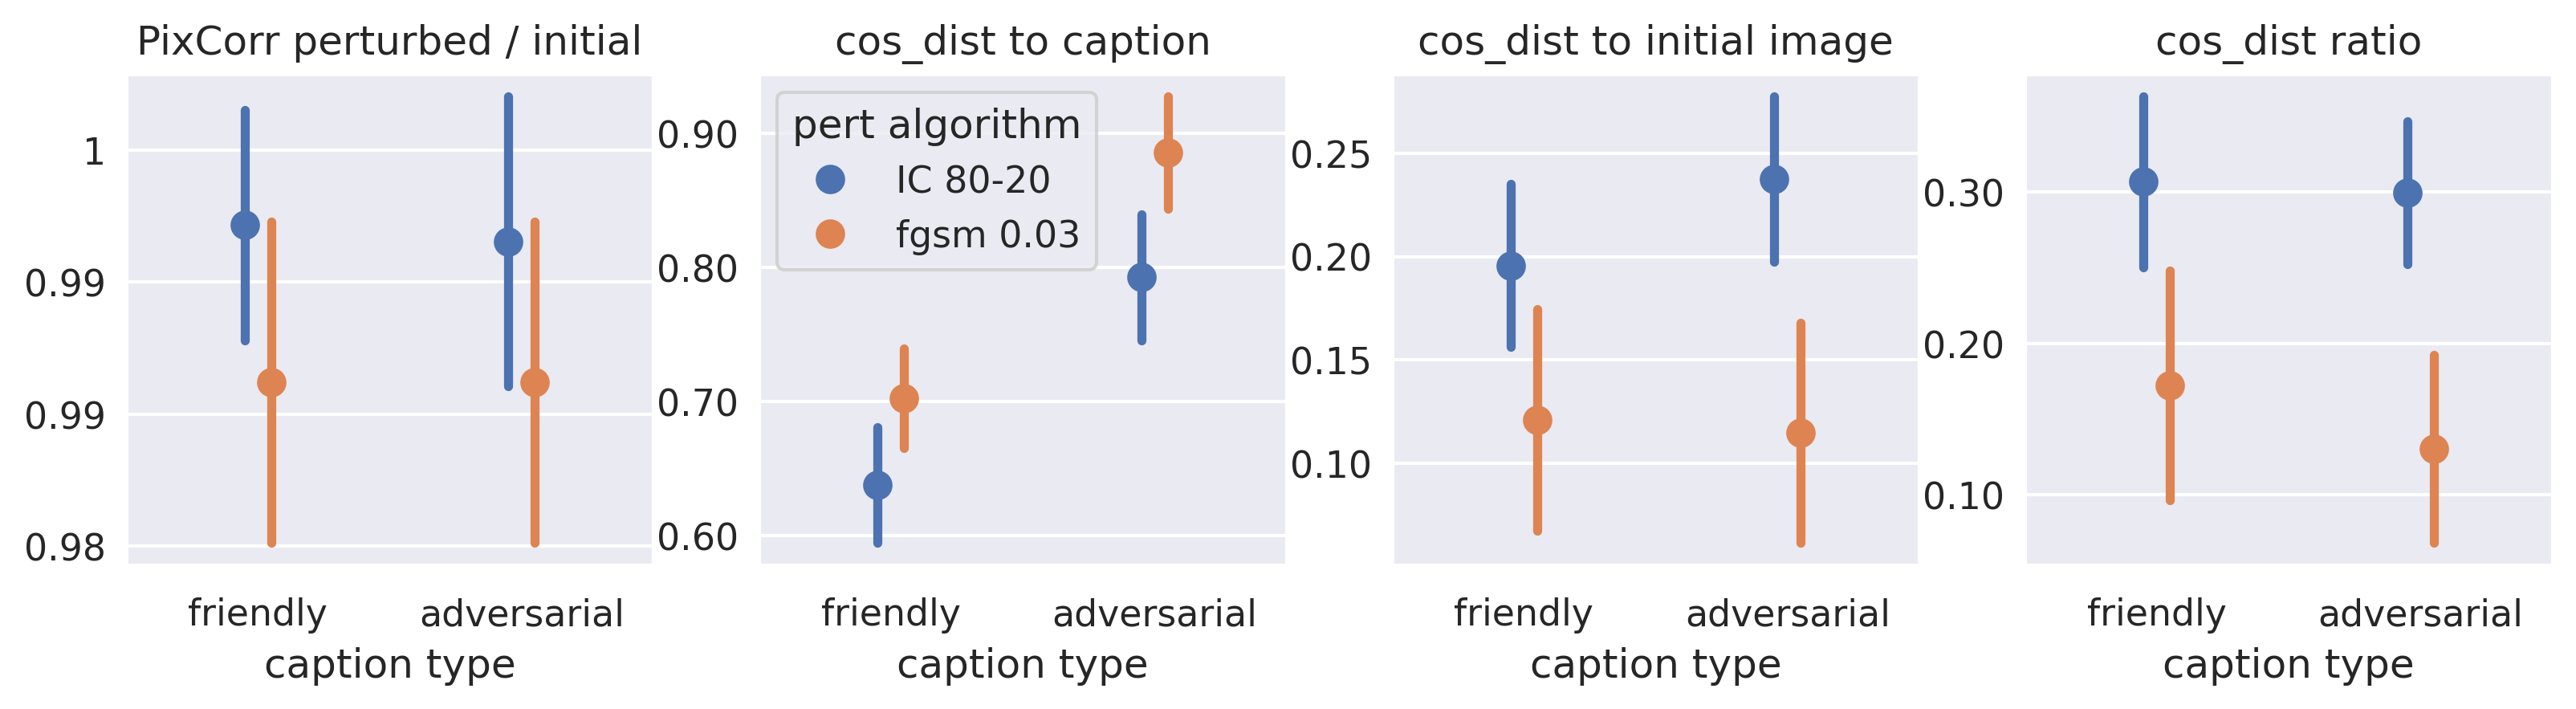
\includegraphics[width=1\textwidth]{plots/advpert_validation_chosen_perts.png}
    \caption[Quantitative Evaluation of FGSM 0.03 vs. IC 80/20]{Quantitative Evaluation of FGSM 0.03 vs. IC 80/20. Perturbation was performed both with IC 80/20 and FGSM 0.03 on all 1200 training samples. Four different criteria are measured for the perturbated images and averaged across all the training samples: The PixelCorrelation of the perturbed and the initial image, the cosine distance of the perturbed image to the caption used for the perturbation process, the cosine distance to the initial image and the ratio of both cosine distances. The results are plotted for both the IC and the FGSM algorithm. The error bars are computed as the standard deviation across all 1200 samples.}\label{fig:advpert_validation_chosen_perts} 
\end{figure}
    
For the reconstruction experiments, five perturbations were created for each of the 1200 training images with the chosen parameters for IC and fgsm: for the friendly perturbations with all five associated captions and for the adversarial perturbations with five different randomly selected captions. This results in a total of 6000 training images. The properties of these 6000 images are compared in Figure~\ref{fig:advpert_validation_chosen_perts}. The IC algorithm produces perturbed images that have, on average, a higher pixel correlation than the fgsm algorithm. In addition, both the cosine distance to the desired perturbation vectors is lower and the cosine distance to the original image is slightly higher than for the fgsm algorithm (resulting in a higher cos dist ratio for the IC algorithm than for fgsm). The IC algorithm has thus better achieved the goal of creating perturbations that visually match the fgsm, but can specifically modify the CLIP Vision embeddings.

% Show some of the images qualitatively that will be shown
\begin{figure}[ht]
    \centering
    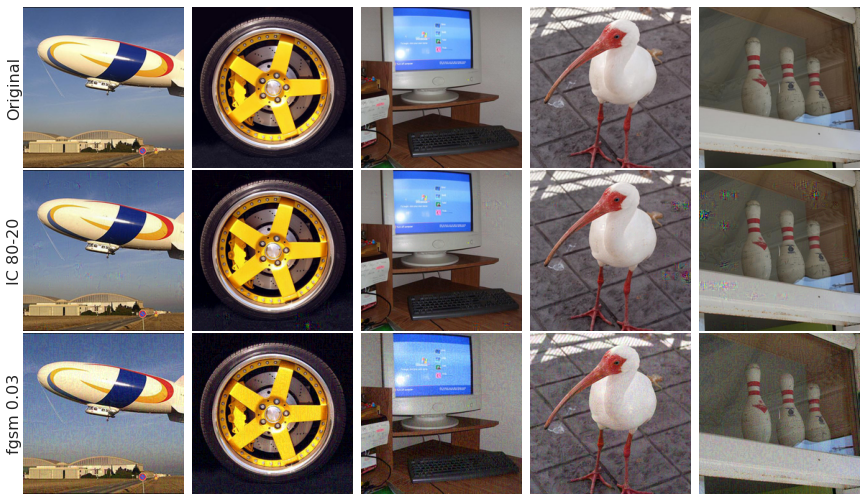
\includegraphics[width=1\textwidth]{plots/advpert_validation_chosen_qual.png}
    \caption[Qualitative Evaluation of FGSM 0.03 vs IC 80/20]{Qualitative Evaluation of FGSM 0.03 vs IC 80/20. For five different training samples, the original image and the perturbated version with FGSM and IC are shown.}\label{fig:advpert_validation_chosen_qual}
\end{figure}

Figure~\ref{fig:advpert_validation_chosen_qual} shows the original and perturbed versions for five images with the two algorithms, as previously shown, the selective artefacts can be seen with IC (particularly visible with the bowling pins) and with fgsm the uniform noise that was superimposed on the image. 

\subsubsection{Changes in the training process}

Now with the perturbed images there are 6000 instead of 1200 training images. However there still are only 1200 averaged MRI recordings (for each image one). The rationale of the perturbation experiment is, that the MRI activation for the perturbed images could be very similar to the perturbed images in comparison to the original images (because they are visually similar). Thus, the 1200 averaged MRI recordings are duplicated 5 times, so that each of the 6000 perturbed images can be predicted by the corresponding MRI activation recording.


\subsection{Results}

As it was shown in the previous section that the IC algorithm achieves the desired perturbation target better than FGSM, the results of the reconstructions with the IC algorithm are described below. The corresponding figures with the FGSM perturbations can be found in the Appendix. Furthermore, the baseline reported in the following results is slightly different from the previous experiments. The ridge parameter of the regression will have a different regularization effect depending on the number of training samples. Since, as described above, the regression for the translator is trained with 6000 images (five different perturbed versions of each input image), each input image for the baseline is also duplicated five times for the baseline, so that the baseline is also trained with 6000 images and the ridge regression treats both the baseline and the experimental conditions the same way. This baseline then would be equivalent to an FGSM with an epsilon of 0. 

\subsubsection{Translator performance}

\begin{figure}[ht]
    \centering
    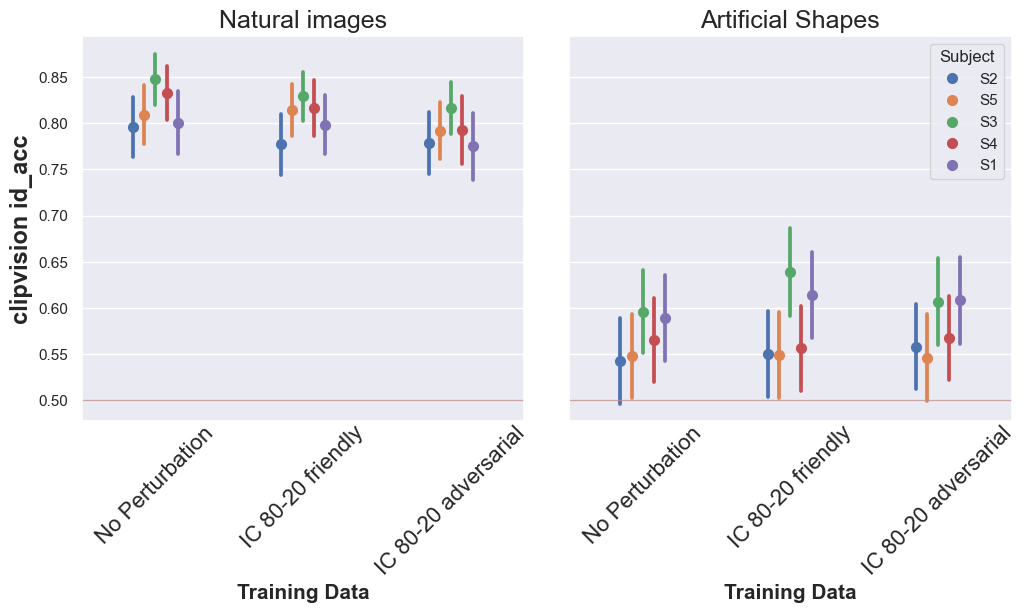
\includegraphics[width=1\textwidth]{plots/advpert_translator_ic_80-20.png}
    \caption[Experiment 3: Translator performance]{Translator performance for friendly and adversarial perturbation with the IC algorithm. The CLIP Vision identification accuracy is displayed for each subject with either no perturbation, friendly perturbation or adversarial perturbation. The results are displayed both for the natural test images and the artificial shapes. The error bars are computed as the standard errors across all test samples.}\label{fig:advpert_translator_ic_80}
\end{figure}

The results of the translator with the perturbed images are shown in Figure~\ref{fig:advpert_translator_ic_80} for both the natural test images and the artificial shapes. The natural test images show that the identification accuracy is lower than the baseline for both the friendly and the adversarial perturbations. This effect seems to be even stronger for the adversarial captions than for the friendly ones. A more ambiguous picture emerges for the artificial shapes. As in the previous experiments, the identification accuracy for the baseline is only slightly higher than the random probability. The perturbed conditions are also only higher than the baseline for some subjects, so it can be assumed that this is a random result. In summary, the perturbations did not lead to any major improvement in the translators. The FGSM showed similar results (see also the figure~\ref{fig:advpert_translator_fgsm_0} in the appendix --- again, the \rOne{translator} showed no improvement over the baseline). 


\subsubsection{Reconstruction performance}

\begin{figure}[ht]
    \centering
    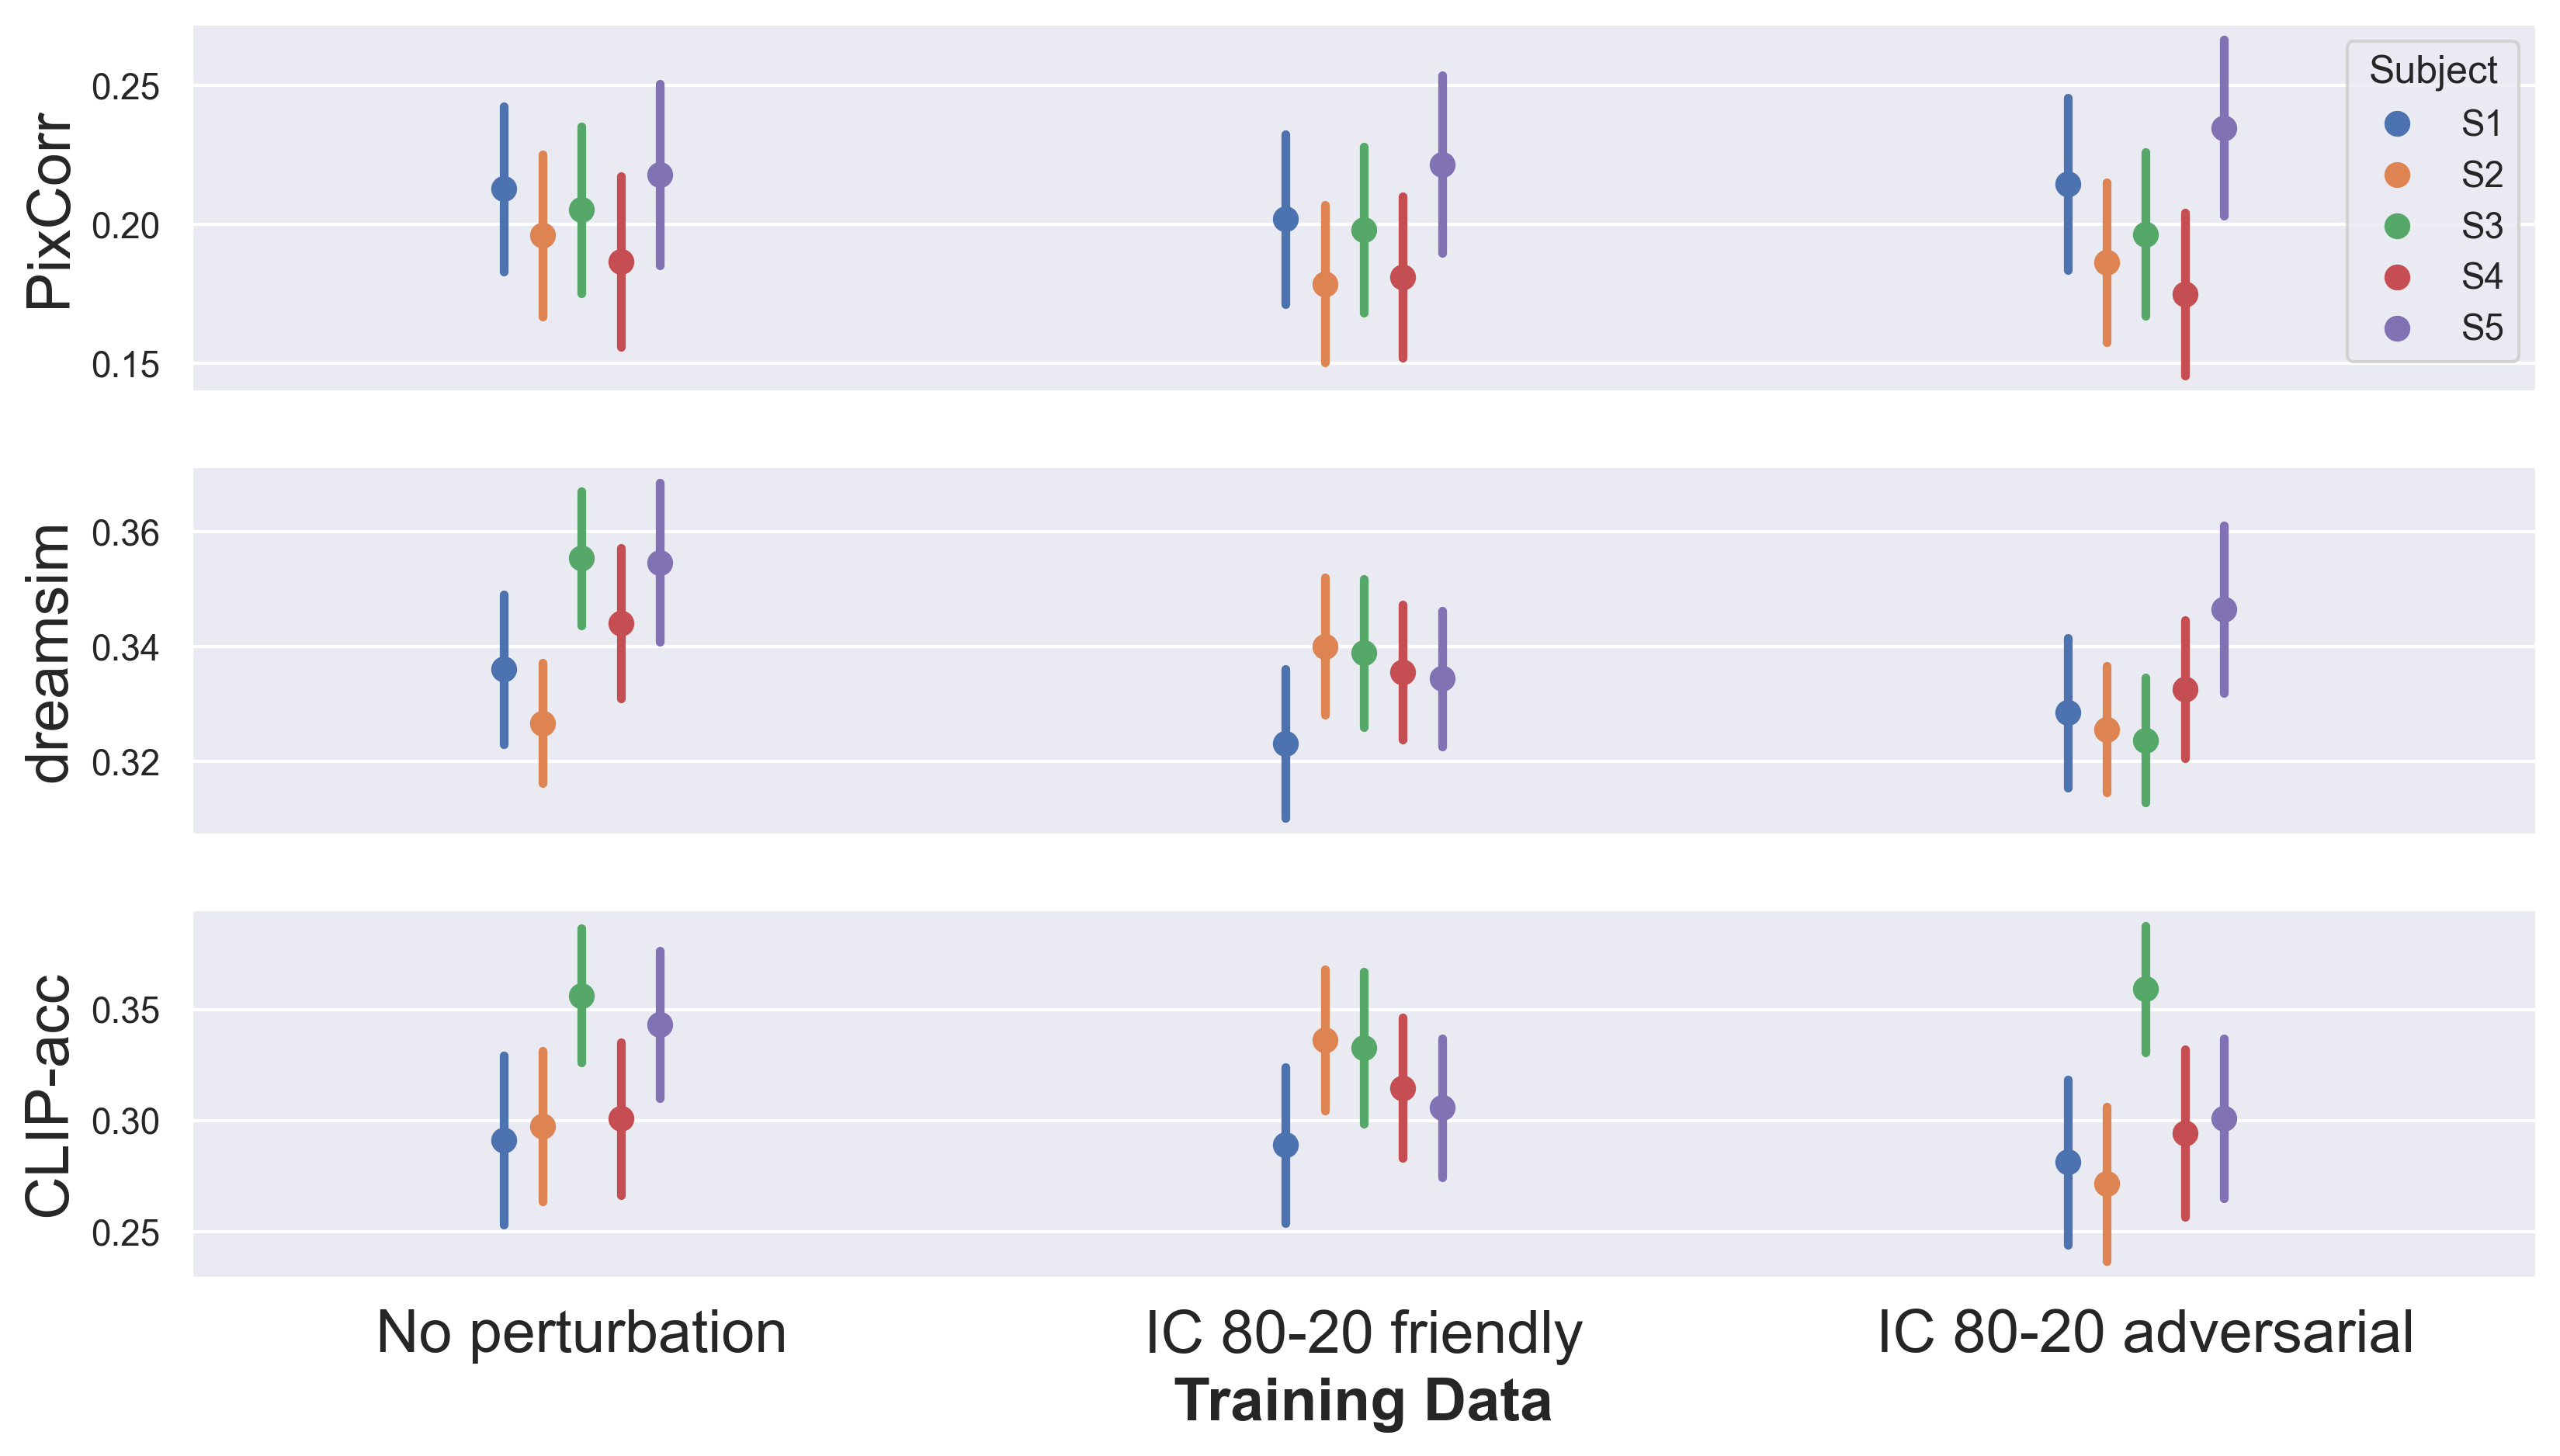
\includegraphics[width=1\textwidth]{plots/advpert_reconstruction_test_ic_80-20.png}
    \caption[Experiment 3: Reconstruction performance on natural test images]{Reconstruction performance on natural test images. The three reconstruction performance criteria (PixelCorrelation, dreamsim and CLIP-accuracy) are displayed for the baseline training dataset and the perturbed dataset with either friendly or adversarial perturbations using the IC 80/20 algorithm. The data is shown for each subject and the error bars are computed as the standard errors across all test samples.}\label{fig:advpert_reconstruction_test_ic_80}
\end{figure}

The results for the reconstruction of the natural test images with the IC algorithm are shown in Figure~\ref{fig:advpert_reconstruction_test_ic_80}.As with the \rOne{translator}, the natural test images show no improvement due to the perturbations. Although the PixelCorrelation results may show a rather good performance, there is a high variance between subjects, especially in the adversarial perturbation condition. The dreamsim indicates a deterioration in the results compared to the baseline, again more so with the adversarial perturbations than with the friendly perturbations. The same pattern can be seen for the CLIP accuracy, with a deterioration in the results that is more pronounced for the adversarial perturbations. The results of the perturbations with FGSM, shown in Figure~\ref{fig:advpert_reconstruction_test_fgsm_0.03} in the appendix, also show no improvement over the baseline. 

\begin{figure}[ht]
    \centering
    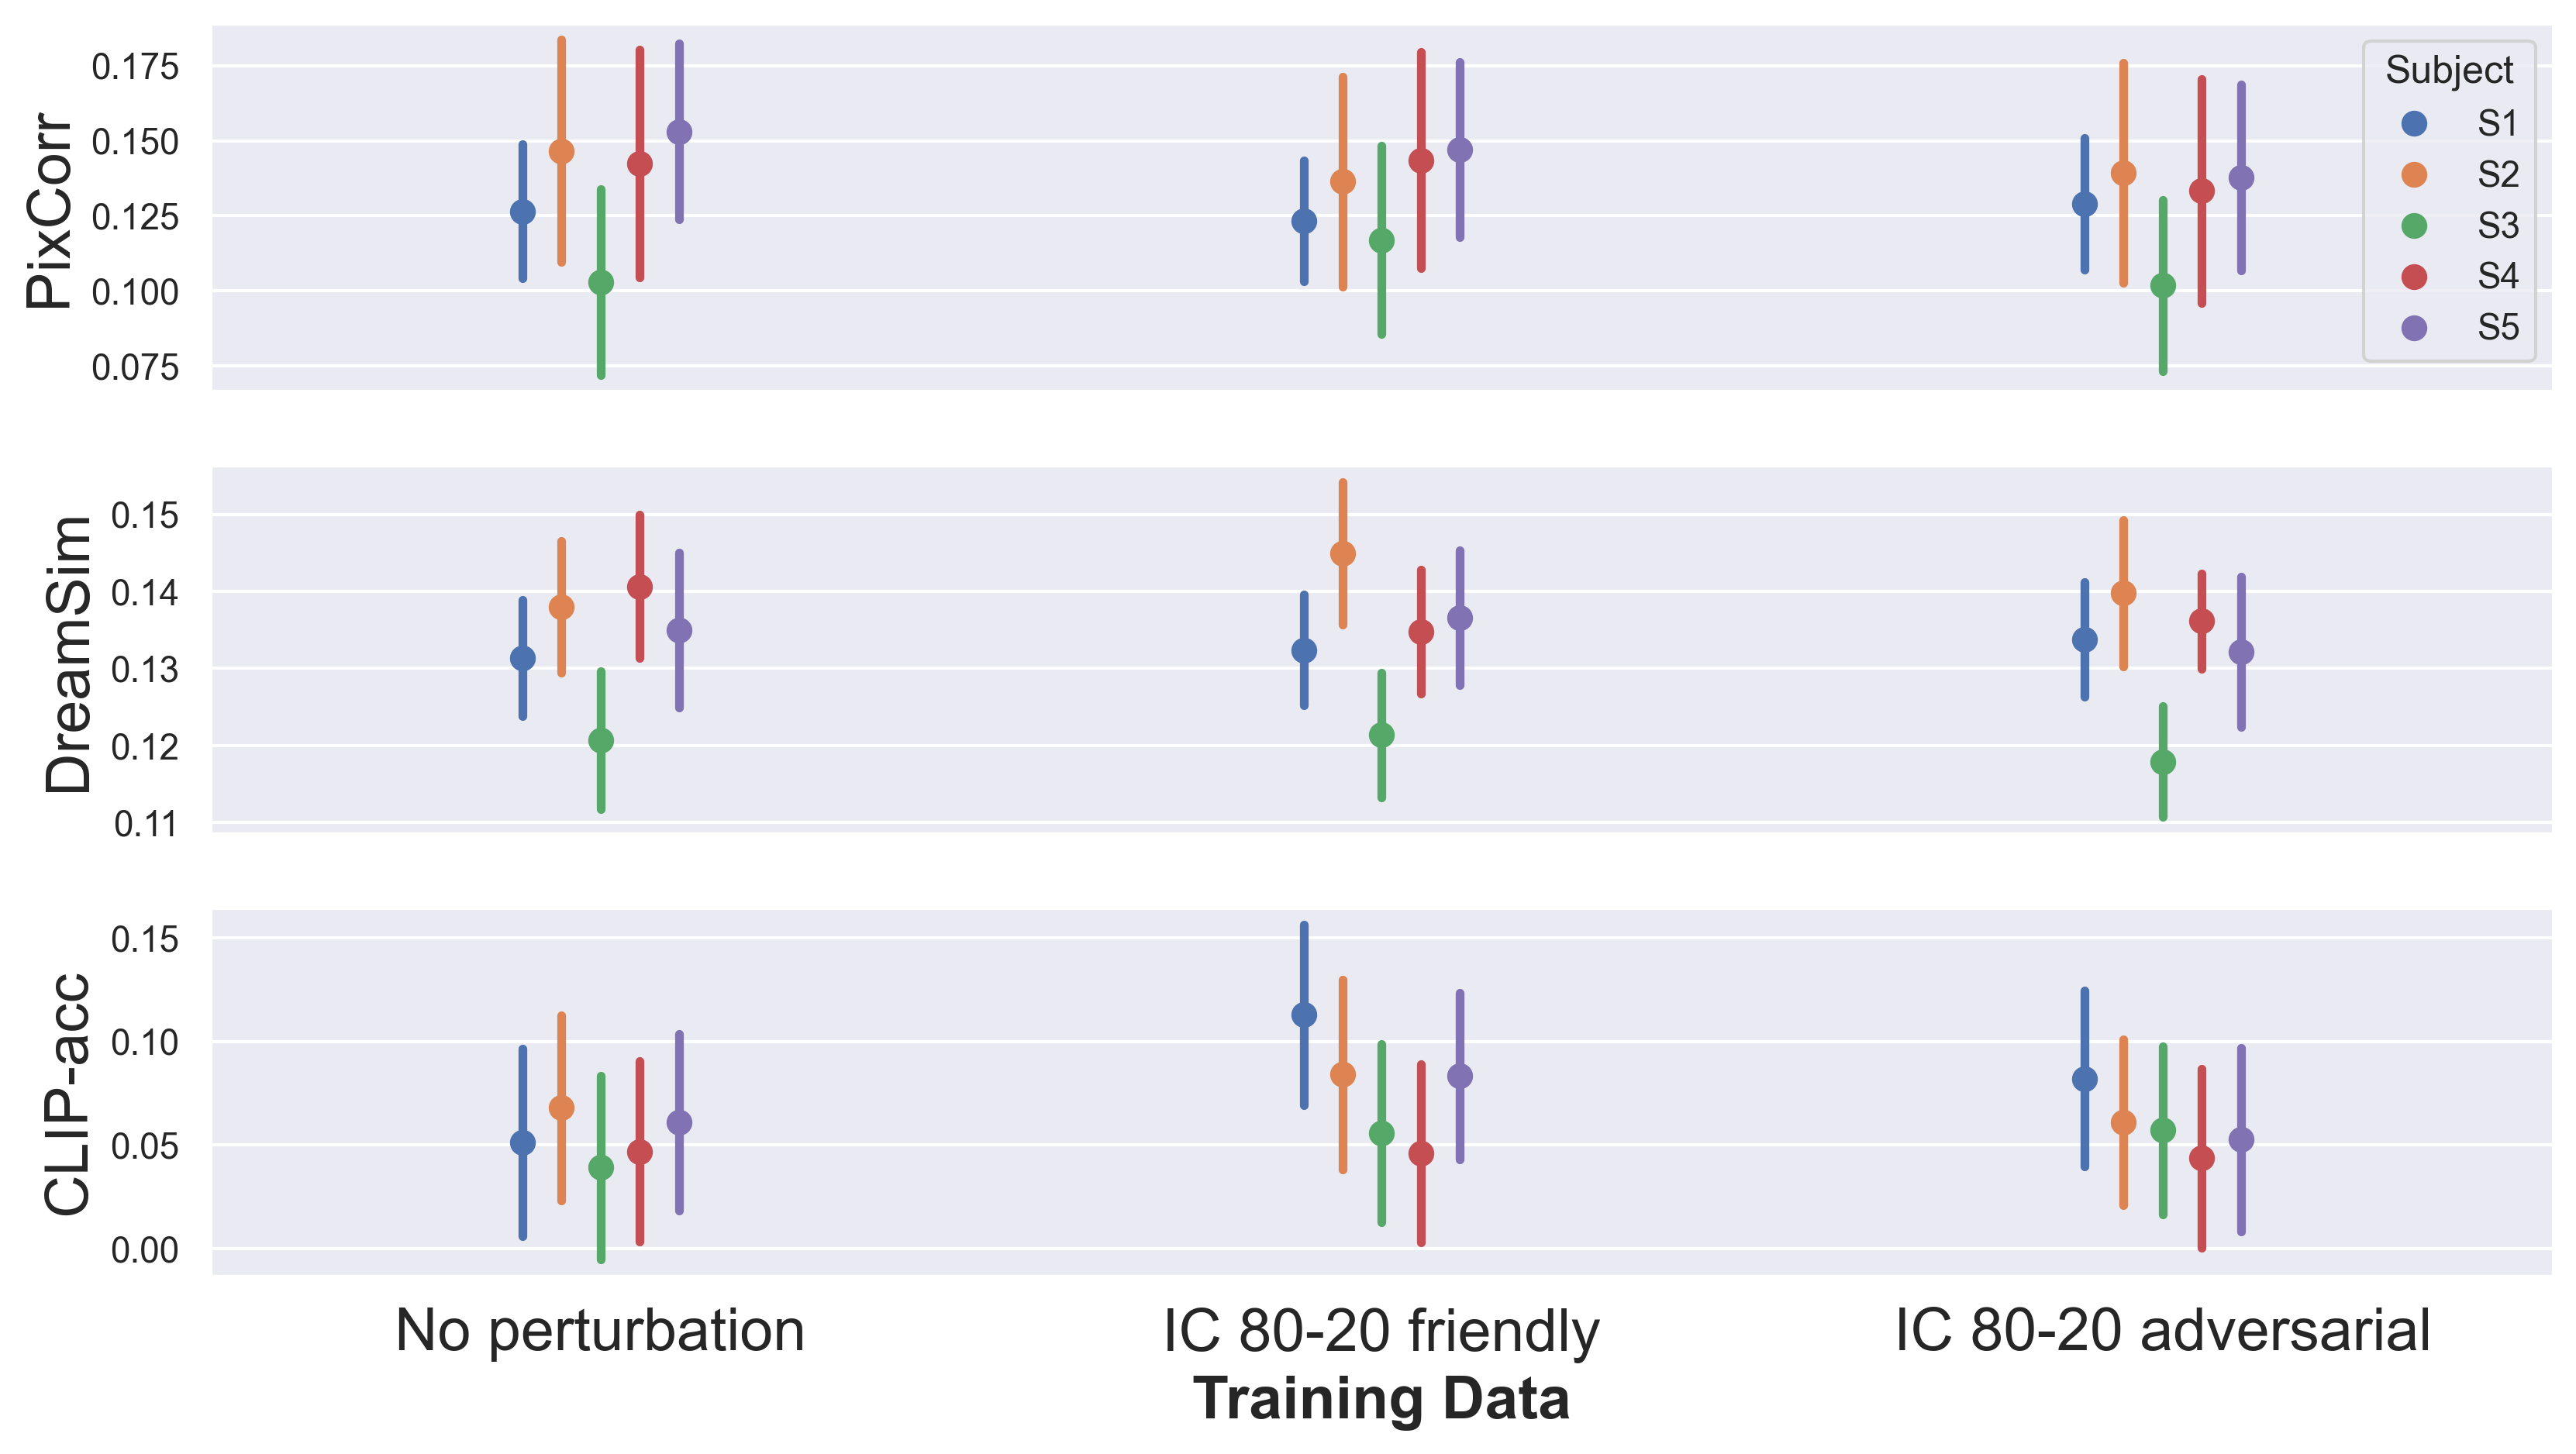
\includegraphics[width=1\textwidth]{plots/advpert_reconstruction_art_ic_80-20.png}
    \caption[Experiment 3: Reconstruction performance on artificial shapes]{Reconstruction performance on artificial shapes. The three reconstruction performance criteria (PixelCorrelation, dreamsim and CLIP-accuracy) are displayed for the baseline training dataset and the perturbed dataset with either friendly or adversarial perturbations using the IC 80/20 algorithm. The data is shown for each subject and the error bars are computed as the standard errors across all test samples.}\label{fig:advpert_reconstruction_art_ic_80}
\end{figure}

The results of the reconstructions of the artificial shapes in Figure~\ref{fig:advpert_reconstruction_art_ic_80} are similar to those of the natural test images. Again, the pixel correlation is difficult to interpret, but tends to be slightly worse for the perturbed images than for the baseline. The results for dreamsim are also ambiguous, but basically show no improvement due to the perturbations. The results for CLIP accuracy are again just above random probability. Again, the perturbed images show no improvement in performance over the baseline. The FGSM results in Figure~\ref{fig:advpert_reconstruction_art_fgsm_0.03} in the appendix also confirm this pattern for the artificial shapes: there is no improvement over the baseline. 

A qualitative evaluation of the images is hard to do because of the very small (and partly negative) differences between the baseline and the perturbated versions. Since there are not many visible differences, a selection of the reconstructed images for both the IC and the fgsm algorithm are displayed in the appendix in figure~\ref{fig:advpert_qual_test} for the natural test images and in figure~\ref{fig:advpert_qual_art} for the artificial shapes.


\subsection{Discussion}
This experiment investigated whether adding perceptually subtle semantic noise to the training images could improve reconstruction performance. Both hypotheses, that friendly perturbations can improve performance for natural test images and that adversarial perturbations can improve performance for artificial shapes, could not be confirmed. The perturbations did not improve the performance of the \rOne{translators} or the reconstructions, but rather slightly worsened it. 

These results are in line with the somewhat ambiguous state of research on this topic described at the beginning of this chapter. With the exception of a few studies that found an improvement in generalisation through adversarial perturbations~\cite{xieAdversarialExamplesImprove2020,yanEnhancingClassificationPerformance2023}, the use of perturbations in augmentation seems to be primarily capable of making classifiers more robust to perturbations instead of helping to generalize the performance of a model~\cite{goodfellowExplainingHarnessingAdversarial2014,madryDeepLearningModels2019}. Another problem with our study is that the same MRI data was used for all five perturbations per training image, so the regression can only learn to predict the mean of all five perturbations for each x-value (MRI measurement). It would be better to have different MRI measurements for each perturbation, but this would violate the goal of not including new MRI data. One possibility would be not to calculate an average of the activity of all presentations in the MRI data, but to pair each MRI activity of a single presentation with a perturbed image. This was also tried in the course of this work, but did not lead to an improvement in performance and is therefore not reported in the results. 

\begin{figure}[ht]
    \centering
    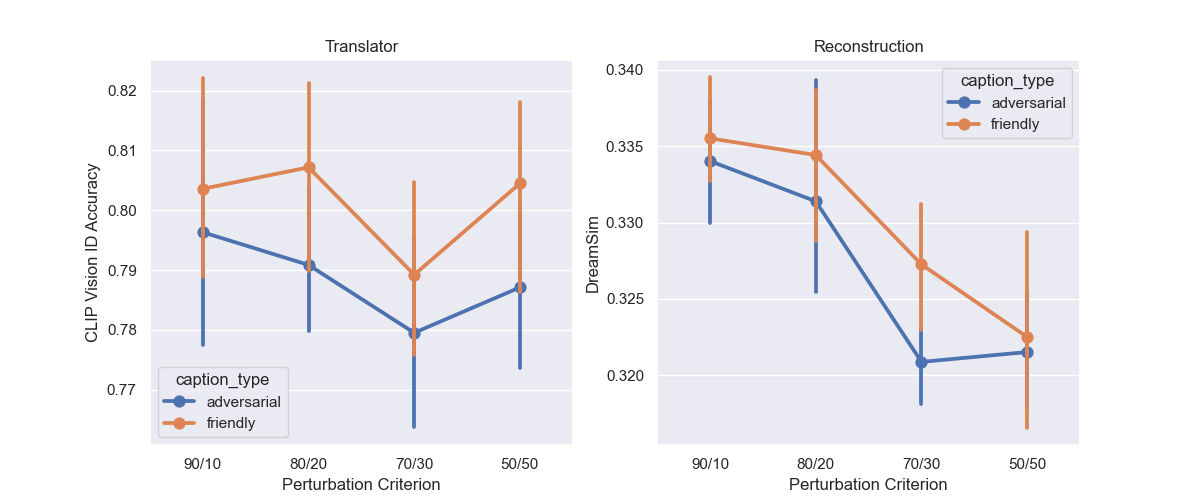
\includegraphics[width=1\textwidth]{plots/advpert_discussion_explore_pert_ratio_test_translator_and_recon.png}
    \caption[Translator/Reconstruction Performance for natural test images with different IC criteria]{Translator and Reconstruction Performance for natural test images with different IC criteria. The translator performance (measured with CLIP Vision identification accuracy) and the reconstruction performance (measured with dreamsim) are displayed for multiple IC criteria with increasing perturbation.}\label{fig:advpert_discussion_explore_pert_ratio_test_translator_and_recon}
\end{figure}

\subsubsection{Future directions}

Since this study aimed not only to explore the effect of perturbations but rather to enrich the training data with semantic information through the perturbation process, there remain opportunities to refine the method to potentially improve performance. For example, different captions could be used to generate the perturbations. In particular, the captions generated for the previous experiment could be used to improve the performance of the artificial shapes by perturbing them with low-level captions. Another direction to explore would be what happens if the perturbations are made even stronger, so that the effect of the CLIP Text captions on the images is greater than that of the CLIP Vision captions. To this end, the effect of an increased IC criterion on performance was investigated in a further experiment, the results of which can be found in Figure~\ref{fig:advpert_discussion_explore_pert_ratio_test_translator_and_recon}. Only the natural test images were used for this, and only the dreamsim is shown for the reconstruction performance. In the graph, the results for all five subjects have been averaged and the error bars describe the standard error across all five subjects. It can be seen that the performance of both the translator and the reconstruction tends to decrease with increasing IC criterion for both adversarial and friendly captions. However, from a very strong perturbation (50/50) there seems to be a positive trend reversal (this is only not visible for the friendly perturbations in the reconstruction performance). It is therefore possible that the performance for the natural test images can be increased again by giving the captions an even stronger influence on the CLIP Vision embeddings. Unfortunately, it was not possible to increase the perturbation ratio any further, as otherwise the IC algorithm would no longer converge and the input images would be perturbed until they were all black. It might be possible to use a better optimisation algorithm here, but as the IC process denormalises the images after each individual step, bringing them into a range of values between 0 and 1, using an optimiser such as ADAM~\cite{kingmaAdamMethodStochastic2017} is not entirely trivial.

Another limitation of the study is the assumption that the response of brain activity to the perturbed images would be very similar to that of the unperturbed images. On the one hand, it is possible that a person's perception, and thus brain activity, can be influenced even if the visual differences cannot be directly identified~\cite{rensinkVisualSensingSeeing2004}. On the other hand, with the IC algorithm, as shown in the method, the result of the perturbation is often that isolated visual artifacts can occur. As salient features in the image, these artefacts could have a strong bottom-up influence on attention and thus on brain activity~\cite{wolfeFiveFactorsThat2017}. This limitation raises the question of whether the conditioning of the perturbation even needs to be guided by minimising the visual differences to the original image. Since the regression is not trained directly on images, but on the CLIP features of the image, it might also be possible to create training data perturbations, which would be much more visually noticeable. As long as the regression can learn to better predict the corresponding CLIP Vision embeddings of the test dataset, it is not directly relevant how much the perturbed images visually differ from the original. Therefore, it might even be an option to make the augmentation of the images completely independent of the visual input and only influence the CLIP Vision space. Backpropagation in the image space would no longer be necessary, so the perturbed feature vector could be moved much more easily in the direction of the CLIP Text embeddings. On another note, in the CLIP Vision context of the versatile diffusion process, all 257 CLIP vectors are used (256 for all ViT patches in the image and one global CLIP vector). The algorithm could possibly deliver better results if the CLIP Vision information about the 256 patches was not distorted, but only the final vector describing the whole image was enriched with the information from the captions. 

